
%%%%%%%%%%%%%%%%%%%%%%%%%
%%%
%%%%%%%%%%%%%%%%%%%%%%%%%
\begin{frame}\frametitle{Neutrino reconstruction}
\centering\footnotesize

Neutrino 4-momentum unknown \\
{\large $\Downarrow$}\\
$\met$ $X$ and $Y$ components + a bit of algebra:\\
$(P_l + P_{\nu})^2 = P_W^2 = M_W^2$\\
{\large $\Downarrow$}\\
two possible $p_{Z_\nu}$ solutions for the 
$Z$ component of the neutrino momentum:\\
$p_{Z_\nu} = \dfrac{\lambda \pm \sqrt{\delta} }{2}$\\

\myskip
Choose the solution giving min$|m_{\rm reco}^{\rm had} - m_{\rm reco}^{\rm lep}|$\\
(this implies also \bjet s association!)

\begin{itemize}
\item If no real solution, $\nu\sim$ collinear to $l \Rightarrow$  $\eta_{\nu}$ set equal to $\eta_{l}$
\end{itemize}

\begin{minipage}{.5\textwidth}\centering
{\scriptsize
\begin{eqnarray*}
\lambda &=& 2\beta \dfrac{p_{Z_l}}{E_l^2-p_{Z_l}^2};\\
\delta  &=& \lambda^2 - 4\gamma;\\
\gamma &=& -\dfrac{\beta^2 - E_l^2 (p_{X_\nu}^2+p_{Y_\nu}^2)}{E_l^2-p_{Z_l}^2}; \\
\end{eqnarray*}
}
\end{minipage}\begin{minipage}{.5\textwidth}\centering
{\scriptsize
\begin{eqnarray*}
\beta  &=& \alpha + p_{X_\nu}p_{X_l} + p_{Y_\nu}p_{Y_l}; \\
\alpha &=& \dfrac{1}{2}(M_W^2 - M_l^2).
\end{eqnarray*}
}
\end{minipage}

\end{frame}



%%%%%%%%%%%%%%%%%%%%%%%%%
%%%
%%%%%%%%%%%%%%%%%%%%%%%%%
\begin{frame}\frametitle{Statistical analyses}
\centering\footnotesize

In the 7~\tev\ analysis three configurations have been tested:

\begin{itemize}
\item \loose\ selection using
$m_{\rm reco}$ and profiling of overall $t\bar{t}$ yield (``\loose'')
\item \tight\ selection 
using $m_{\rm reco}$ (``\tight'')
\item \tight\ selection  considering just the overall yield and not 
the shape of $m_{\rm reco}$ (``\tight\ cut-and-count'')
\end{itemize} 

Look at expected value of $CL_{\rm s}$ as a function of $m_{\T}$ for best performance:\\

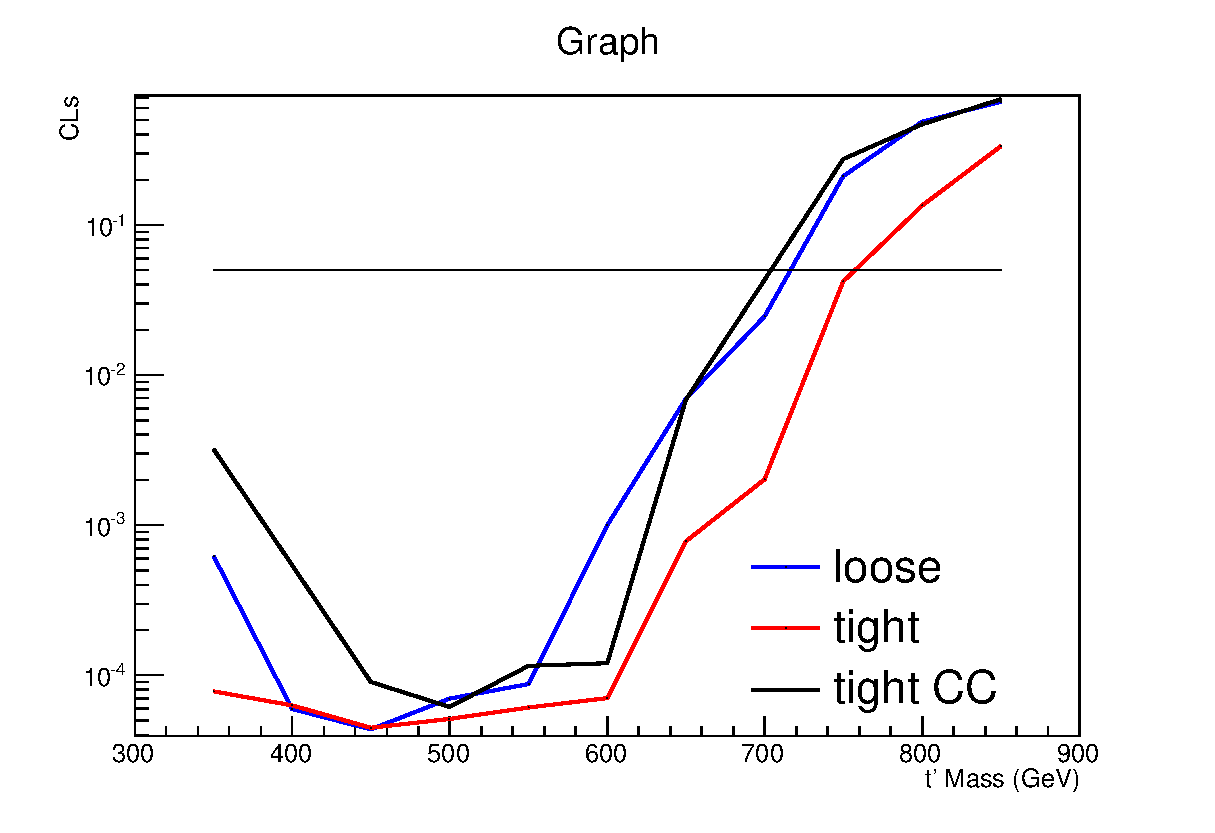
\includegraphics[width=.6\textwidth]{pics/CLs_versus_Mass}


\end{frame}



%%%%%%%%%%%%%%%%%%%%%%%%%
%%%
%%%%%%%%%%%%%%%%%%%%%%%%%
\begin{frame}\frametitle{Generator choice for \ttbar}
\centering\footnotesize

Comparison data to background prediction w/ different \ttbar\ generators\\
e.g. in SDR3 ({\sl loose} selection with reversed $b$-jet $\pt$ cuts)\\
\myskip

\begin{minipage}{.33\textwidth}\centering
\texttt{MC@NLO}\\
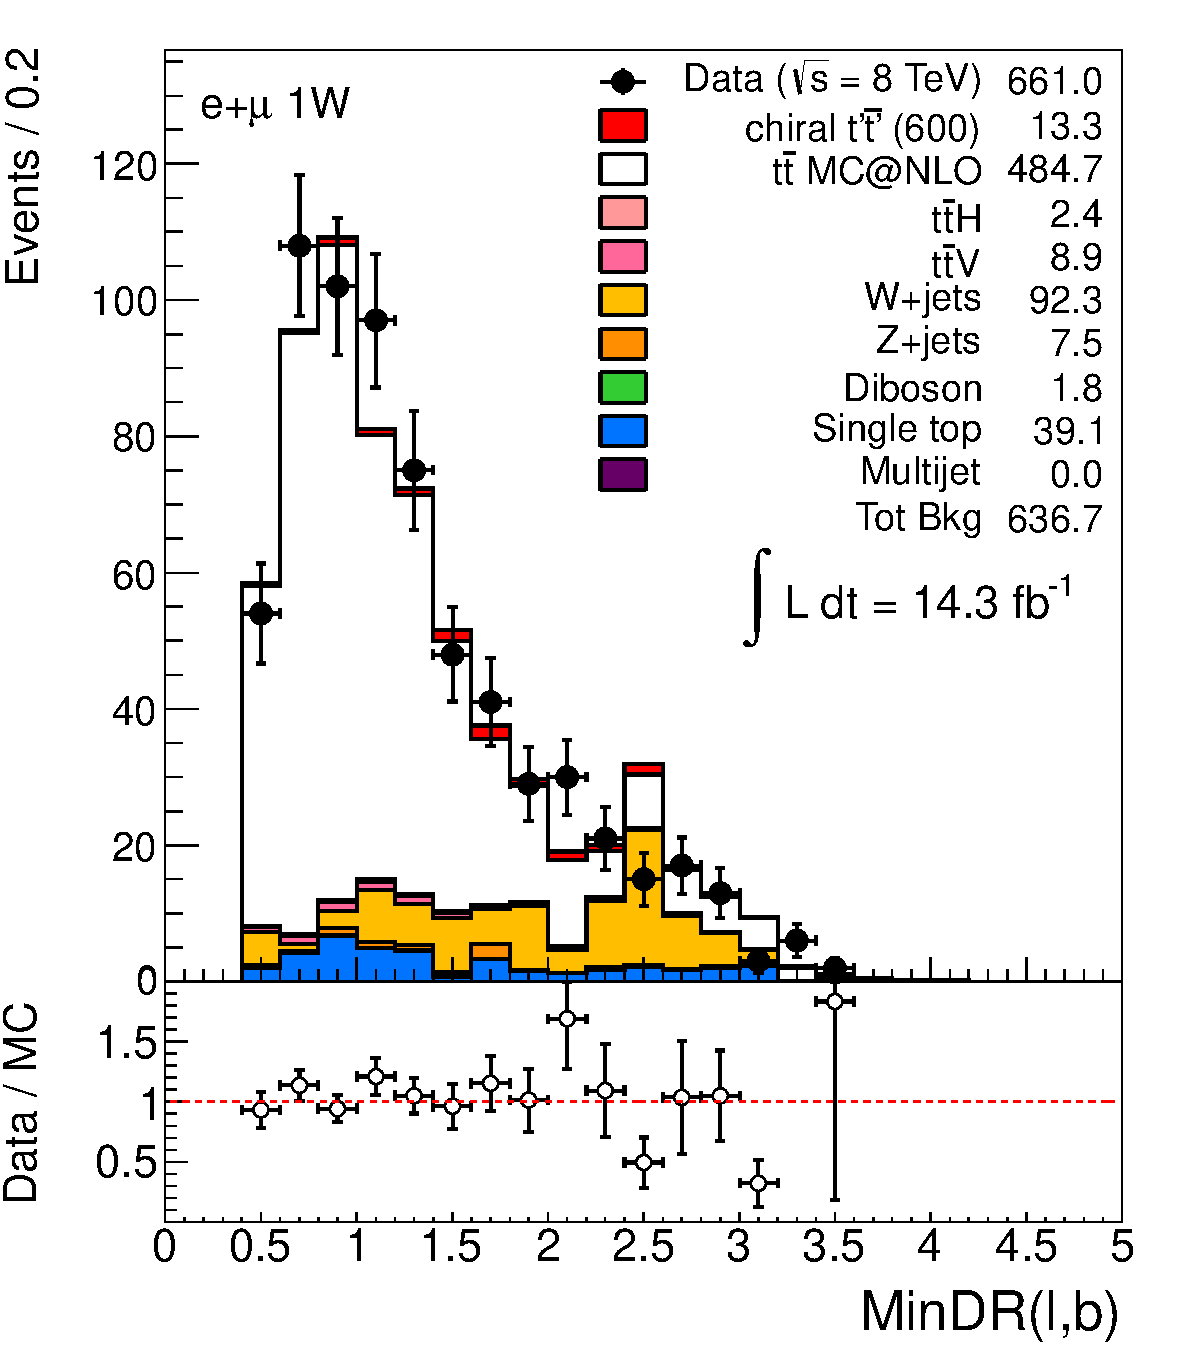
\includegraphics[width=0.9\textwidth]{pics/wbxgen/ttbar5200/VLQAna_WbX_MinDRlb_ELEMUONCR2_1W_NOMINAL}

\end{minipage}\begin{minipage}{.33\textwidth}\centering
\texttt{POWHEG+PYTHIA} \\
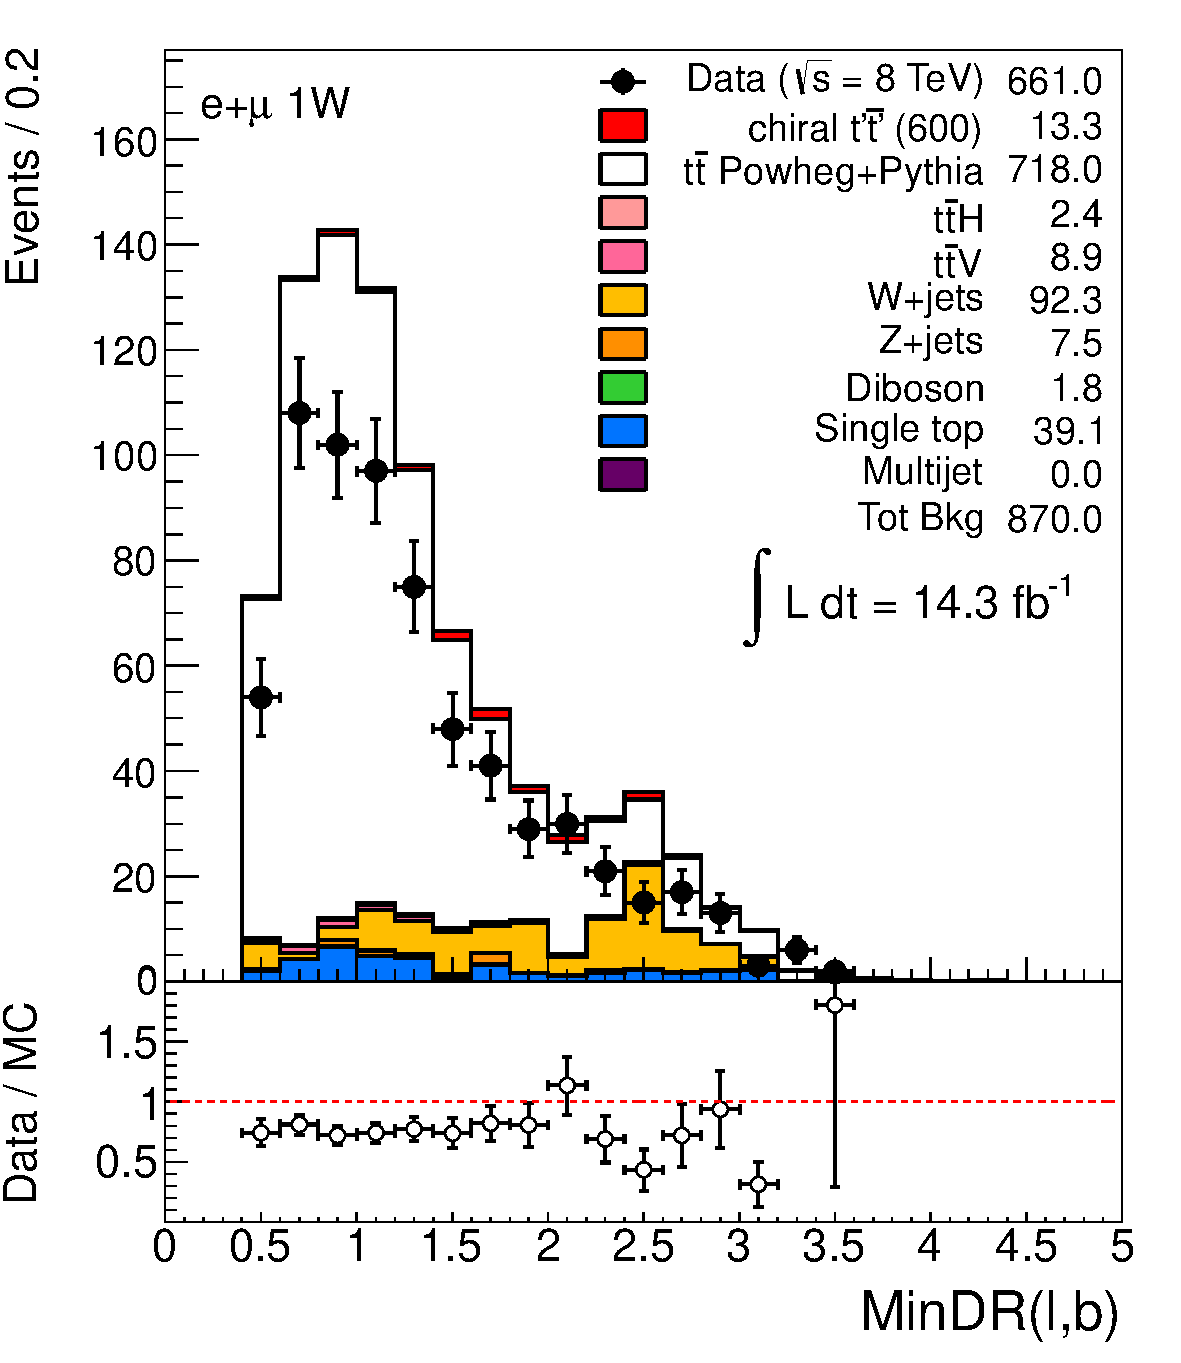
\includegraphics[width=0.9\textwidth]{pics/wbxgen/ttbar117050/VLQAna_WbX_MinDRlb_ELEMUONCR2_1W_NOMINAL}


\end{minipage}\begin{minipage}{.33\textwidth}\centering
\texttt{ALPGEN+HERWIG}\\
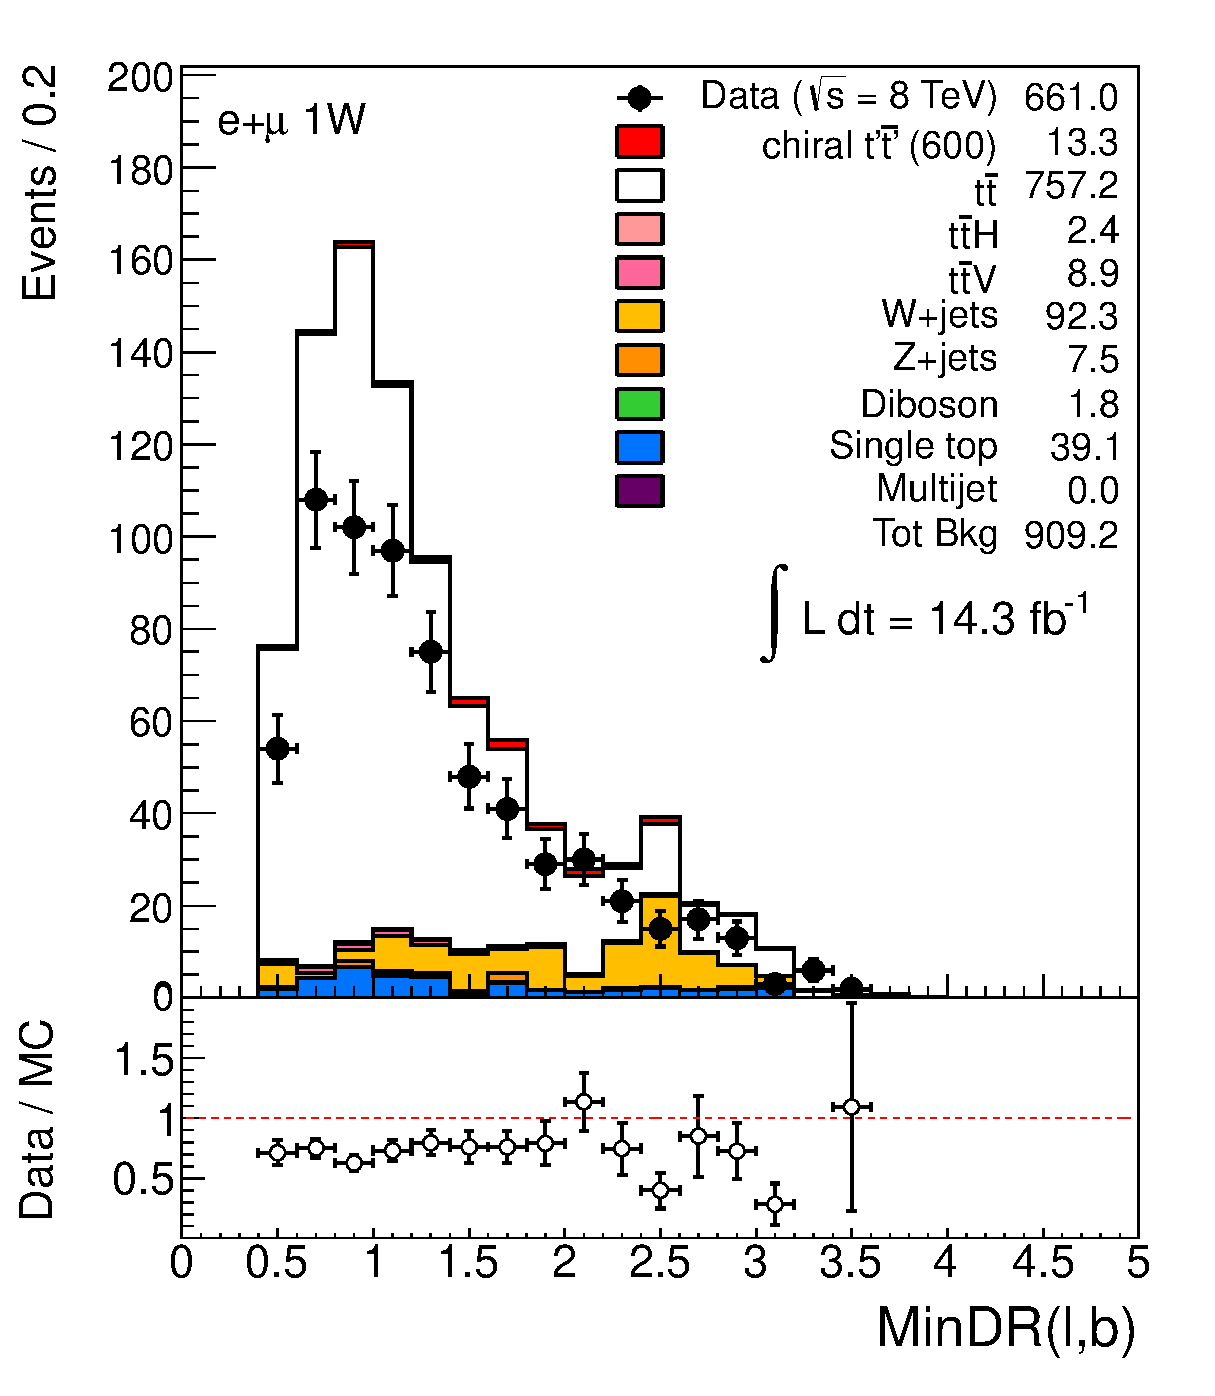
\includegraphics[width=0.9\textwidth]{pics/wbxgen/ttbarAlpgen_HFOR/VLQAna_WbX_MinDRlb_ELEMUONCR2_1W_NOMINAL}


\end{minipage}


\end{frame}


%%%%%%%%%%%%%%%%%%%%%%%%%
%%%
%%%%%%%%%%%%%%%%%%%%%%%%%
\begin{frame}\frametitle{\ttbar\ modeling systematic uncertainties}
\centering\footnotesize

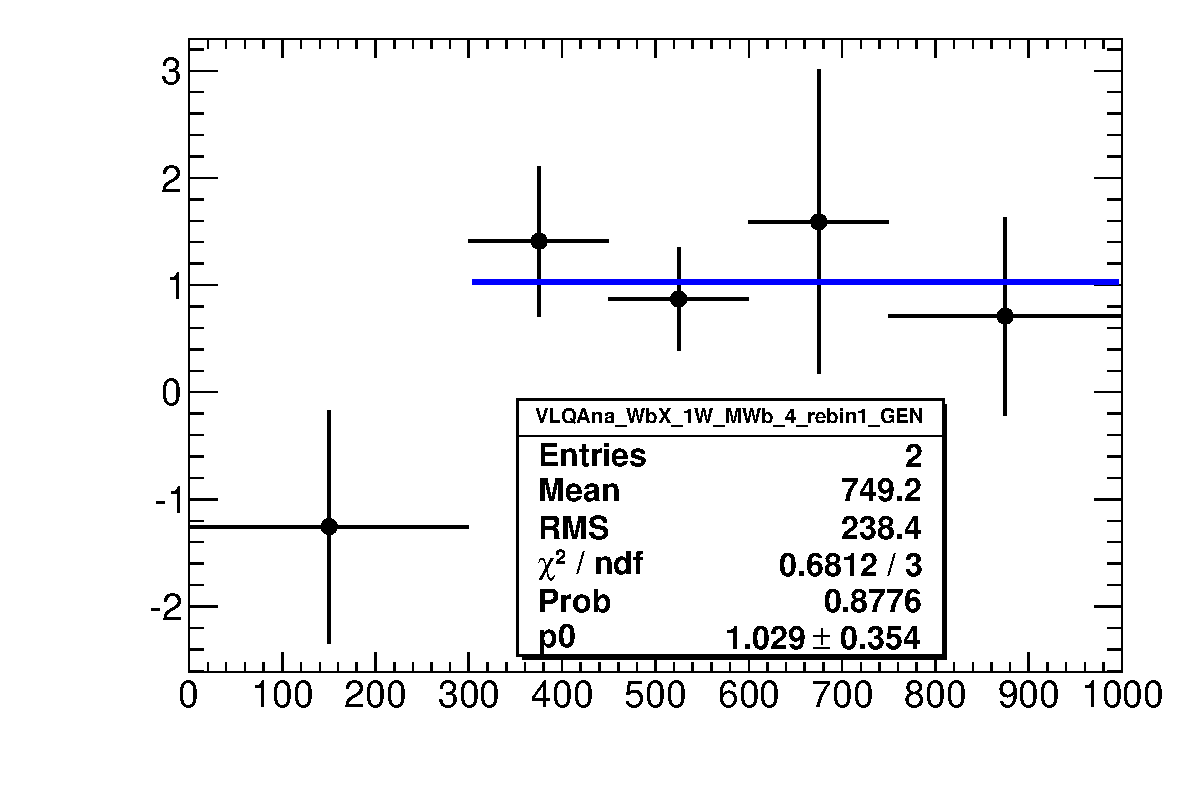
\includegraphics[width=.33\textwidth]{pics/GEN_RATIO.pdf}
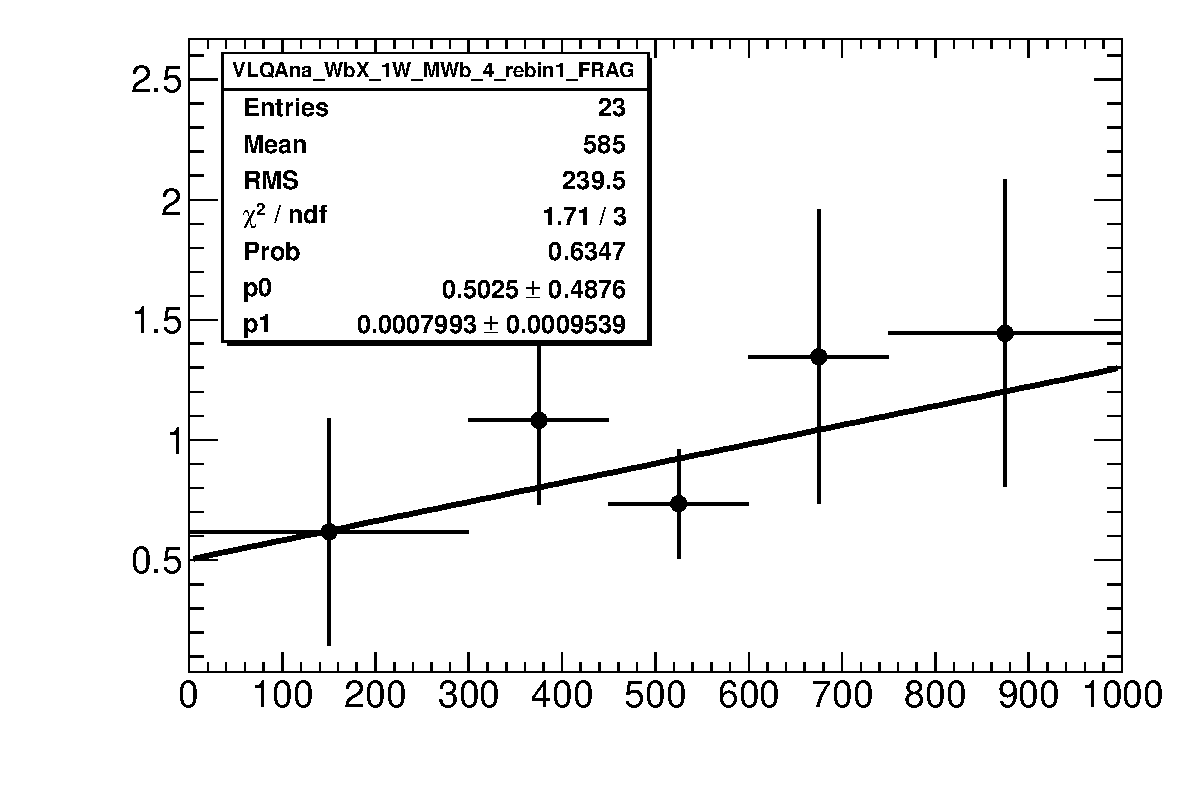
\includegraphics[width=.33\textwidth]{pics/FRAG_RATIO.pdf}
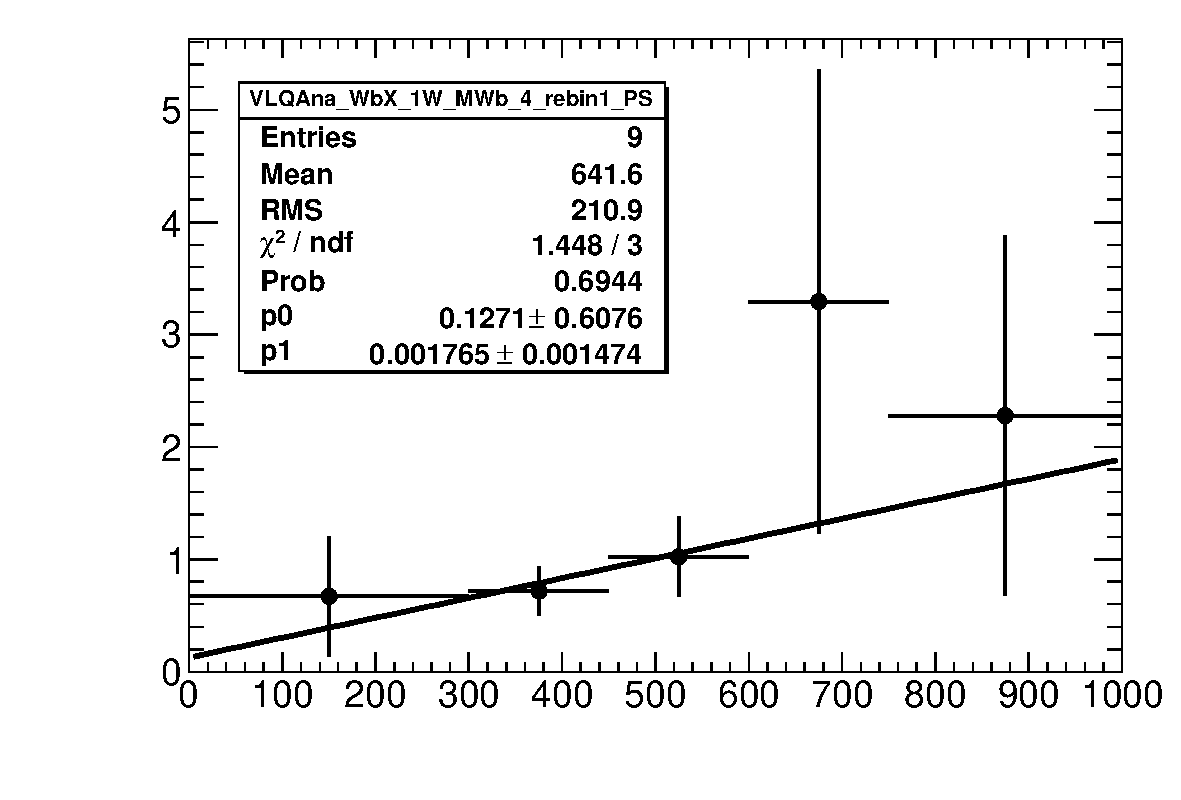
\includegraphics[width=.33\textwidth]{pics/PS_RATIO.pdf}

\end{frame}


%%%%%%%%%%%%%%%%%%%%%%%%%
%%%
%%%%%%%%%%%%%%%%%%%%%%%%%
\begin{frame}\frametitle{Most relevant systematic uncertainties}
\centering\footnotesize

\begin{tabular}{l*{3}{c}}
\toprule
 & $\T\bar{\T}$ ($600\gev$) & $t\bar{t}$ & Non-$t\bar{t}$\\
\midrule
Total [\%] & +14/-15 & +59/-59 & +42/-35\\
\midrule
Main contributions [\%] &&&\\
Jet energy scale & +6.6/-8.4 & +15/-15 & +33/-22\\  
$t\bar{t}$ modelling: NLO MC generator & -- & +48/-48 & --\\  
$t\bar{t}$ modelling: PS and fragm & -- & +25/-25 & --\\  
$t\bar{t}$ modelling: ISR/FSR & -- & +8.8/-8.8 & --\\   
\bottomrule
\end{tabular}

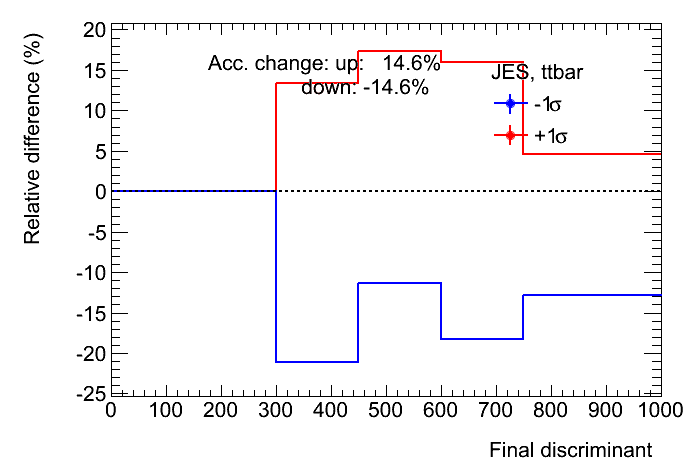
\includegraphics[width=.4\textwidth]{pics/ELEMUON_tight_Bin1_ttbar_JES.png}
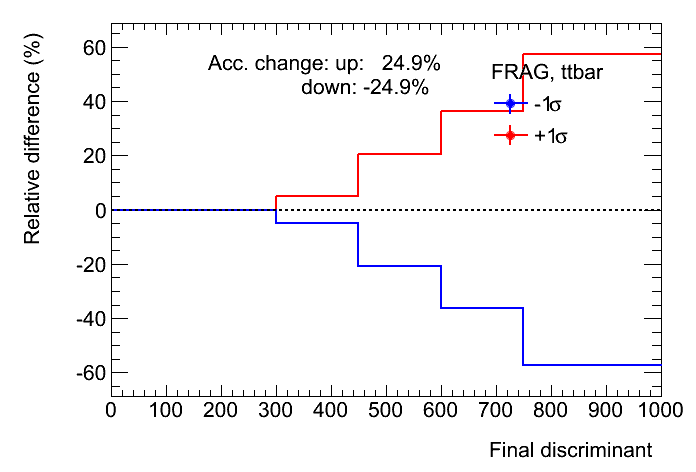
\includegraphics[width=.4\textwidth]{pics/ELEMUON_tight_Bin1_ttbar_FRAG.png}


\end{frame}


%%%%%%%%%%%%%%%%%%%%%%%%%
%%%
%%%%%%%%%%%%%%%%%%%%%%%%%
\begin{frame}\frametitle{\dots updating 7~\tev\ results}
\centering\footnotesize

\begin{minipage}{.5\textwidth}\centering
First model-independent search\\

{\cccolor {\it Phys.Lett.} {\bf B718} (2012)~\cite{ATLAS:2012qe}}

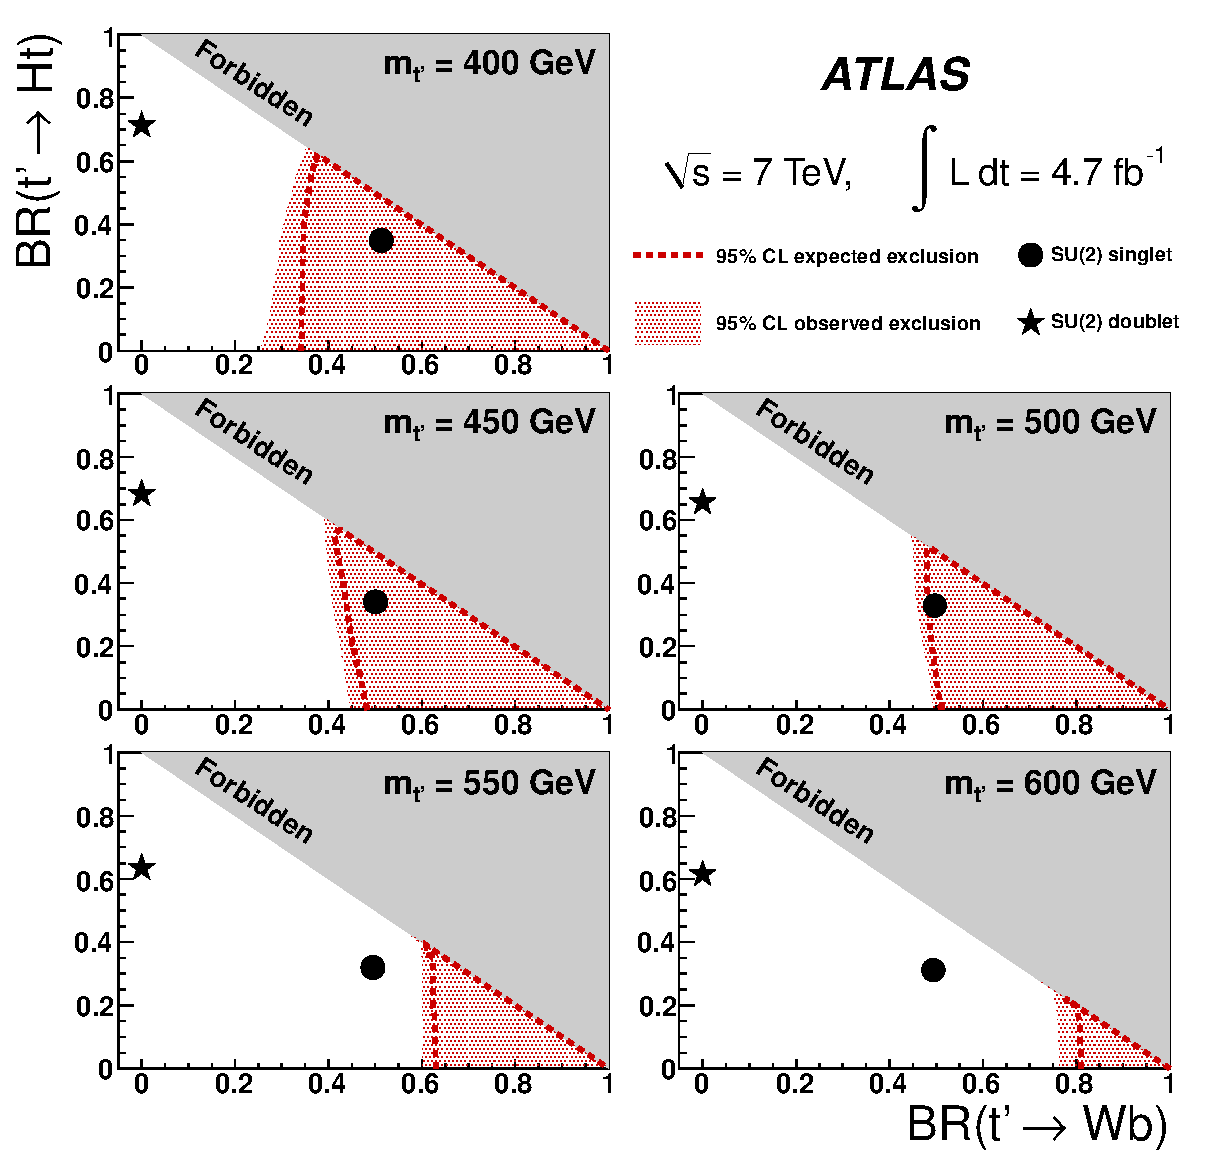
\includegraphics[width=1.\textwidth]{../appendices/figures/wbwb/fig_04}

\end{minipage}\begin{minipage}{.5\textwidth}\centering

\myskip\scriptsize

8~\tev\ analysis: tighter cuts, higher mass points

\myskip
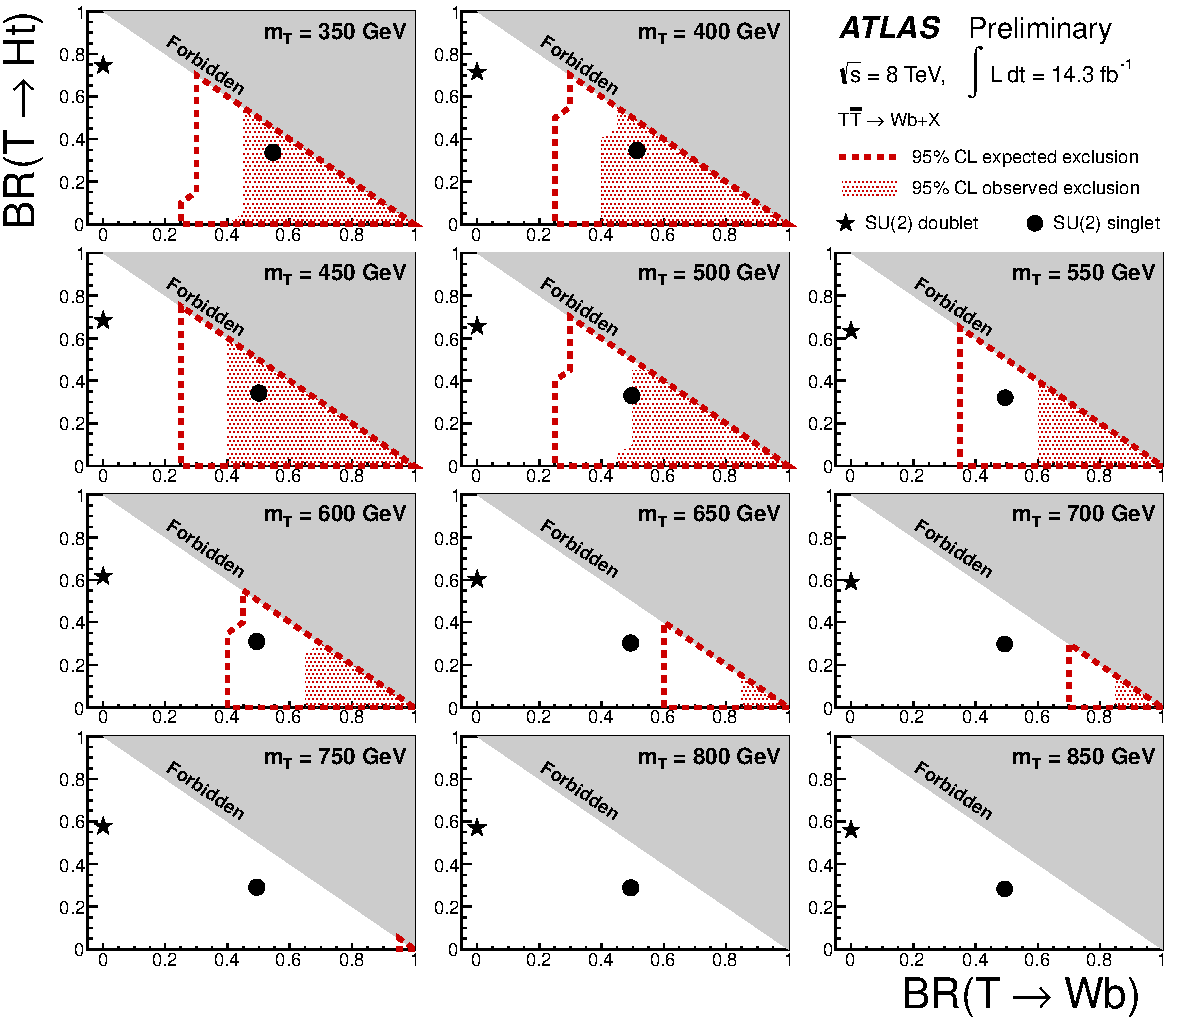
\includegraphics[width=1.\textwidth]{pics/lim_Scan2D_tight_Bin1.pdf}

\end{minipage}



\end{frame}
